\begin{figure}[t!]
    \centering
    \captionsetup{type=figure}
    \begin{subfigure}[t]{0.48\linewidth}
        \centering
        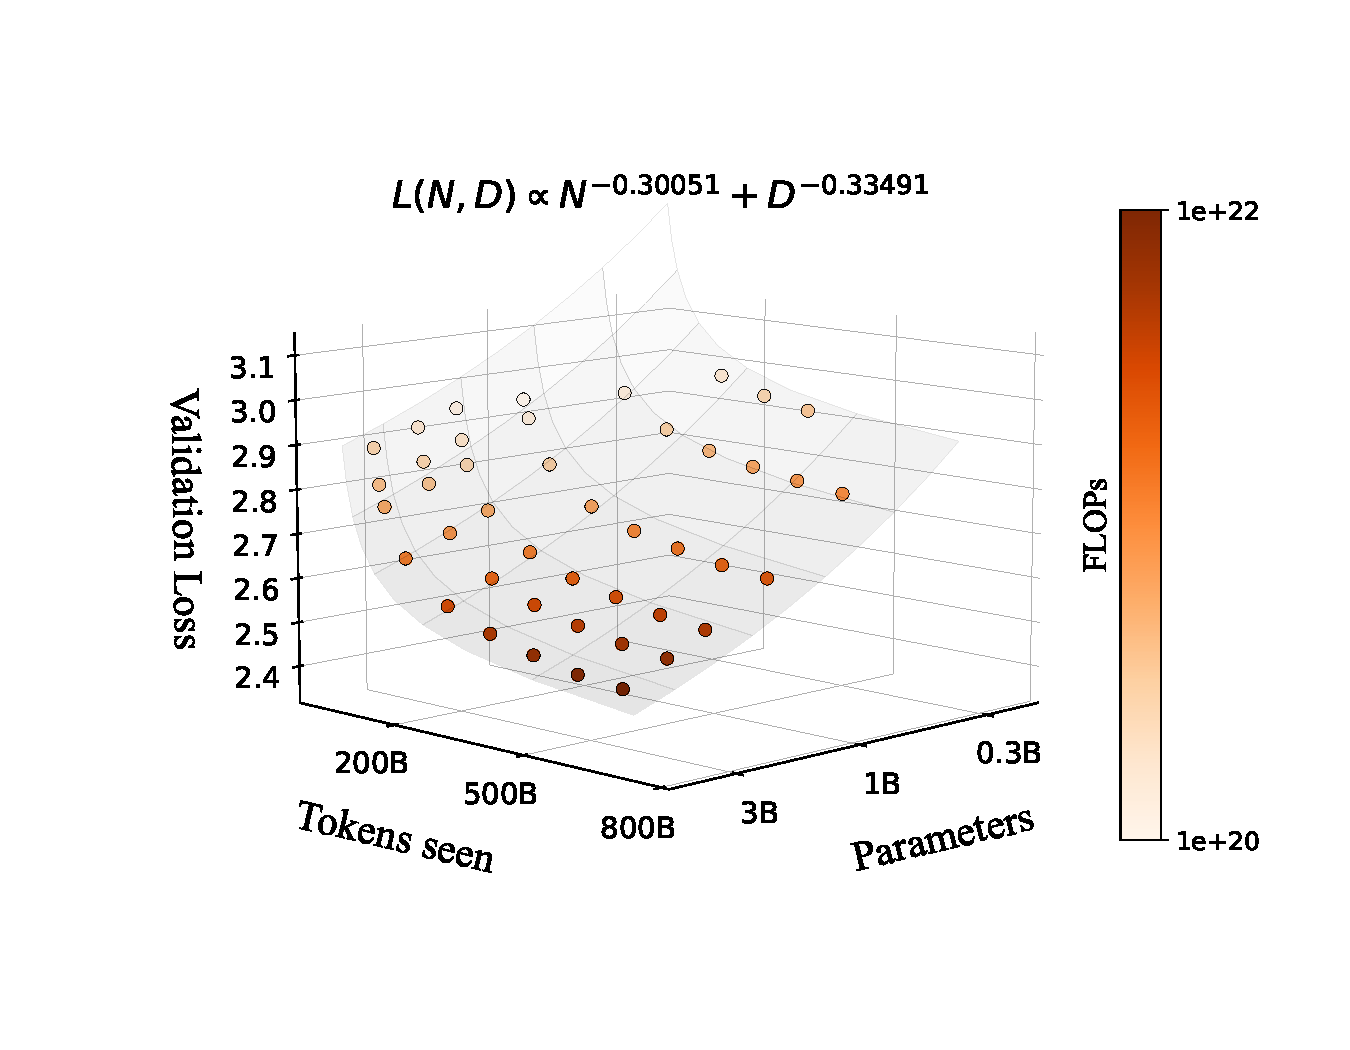
\includegraphics[width=1.02\linewidth]{assets/early/3d_scaling_early.pdf}
    \end{subfigure}
    \hfil
    \begin{subfigure}[t]{0.48\linewidth}
        \centering
        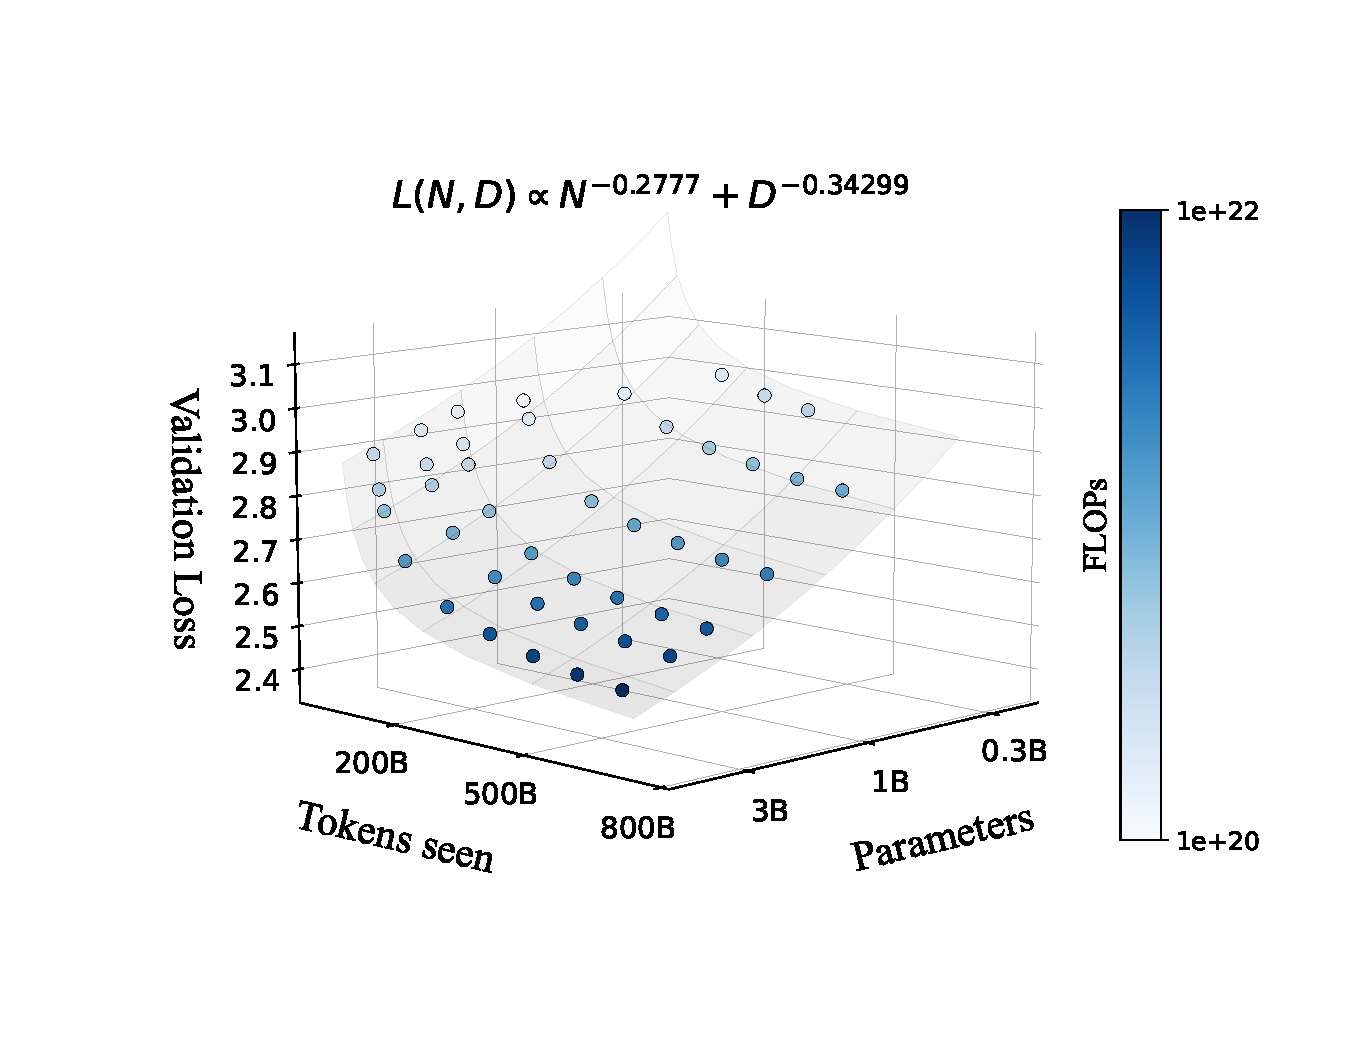
\includegraphics[width=1.02\linewidth]{assets/early/3d_scaling_late.pdf}
    \end{subfigure}
    \vspace{5pt}
    \setlength{\fboxsep}{0.5pt}
    \setlength{\fboxrule}{0pt}
    \caption{\textbf{原生多模态模型中 \fbox{\colorbox{CustomC_Light1!20}{\strut early-fusion}} 与 \fbox{\colorbox{CustomD_Light1!20}{late-fusion\strut}} 的尺度规律。} 每个点表示一个在不同 \edit{数量的} tokens(250M 到 400B)上训练的模型(300M 到 3B 参数)。我们报告了在 \edit{交错数据(Obelics)、图像描述数据(HQITP)和纯文本数据(DCLM)} 的验证集上的平均交叉熵损失。}
    \label{fig:early_vs_late_scaleflops_3d}
\end{figure}
